\documentclass[10pt,a4paper]{article}
\usepackage[margin=2cm]{geometry}
\usepackage{amsmath,amssymb,bm}
\usepackage{graphicx}
\usepackage{booktabs,tabularx,array}
\usepackage{float}
\usepackage[font=small,labelfont=bf]{caption}
\usepackage{xcolor}
\usepackage{adjustbox}
\usepackage{enumitem}
\usepackage[colorlinks=true,linkcolor=blue!50!black,urlcolor=blue!50!black]{hyperref}

\newcommand{\el}{\ensuremath{e^-}}
\newcommand{\AGMX}{A\_GMX}
\newcommand{\code}[1]{\texttt{#1}}
\newcommand{\N}{\mathcal{N}}
\renewcommand{\arraystretch}{1.12}
\setlength{\parskip}{3pt}
\setlength{\parindent}{0pt}
\setlist{itemsep=1pt,topsep=2pt}
\setlength{\emergencystretch}{3em}

\title{\textbf{A\_GMX in brief}\\[3pt]\large the algorithm as implemented, and the comparison with WADERs}
\author{comm\_scripts clustering study}
\date{code of 26 October 2026}

\begin{document}
\sloppy
\maketitle

\noindent\small Code: \code{clustering\_tests/adaptive.py} (\code{adaptive\_cluster(..., engine="gmx")}),
\code{clustering\_tests/gmx.py} (\code{general\_cluster}), \code{clustering\_tests/agent\_methods.py}
(\code{background\_map}), \code{clustering\_tests/fe\_candidates.py}; run with \code{run\_AGMX} or
\code{run\_WADERs --clusterer agmx}. The full derivations, the history and every test are in
\code{docs/aGMX/aGMX\_clustering.pdf}.\normalsize

%======================================================================================================
\section{Input, output, notation}

Input: a calibrated image $Q_p$ in electrons (panaSKImg's \code{*\_EXT<n>\_waders.fits.bz2}, converted with the
module's $g(n)$ curve) and its active-pixel mask. Output: one record per cluster (energy, position, width, class,
quality flags, pixels with the charge taken from each) in the WADERs ROOT format, and for electron-counting CCDs a
few-electron candidate catalogue. Energy $=$ charge $\times$ 3.74\,eV/\el.

Pixel model: $Q_p=o_p+n_p+\epsilon_p+D_p$ with offset $o_p$, dark charge $n_p\sim\mathrm{Poisson}(\lambda_p)$, read
noise $\epsilon_p\sim\N(0,s_p^2)$ and deposit charge $D_p$. Derived maps: $R_p=Q_p-o_p-\lambda_p$ (residual),
$V_p=\lambda_p+s_p^2$ (variance of an empty pixel), $R^+_p=\max(R_p,0)$.

%======================================================================================================
\section{The algorithm}
The figures of this section show each step on one real image: a low-background Am-241 CCD image (AMTEst EXT1,
0.12\,\el{} read noise) with eleven known deposits injected in a quiet region (figure~\ref{fig:scene}), clustered by
the current code (\code{clustering\_tests/make\_agmx\_figures.py}, \code{AGMX\_FIG\_OUT=figures\_current
MUON\_PHYS=1}).

\begin{figure}[H]\centering
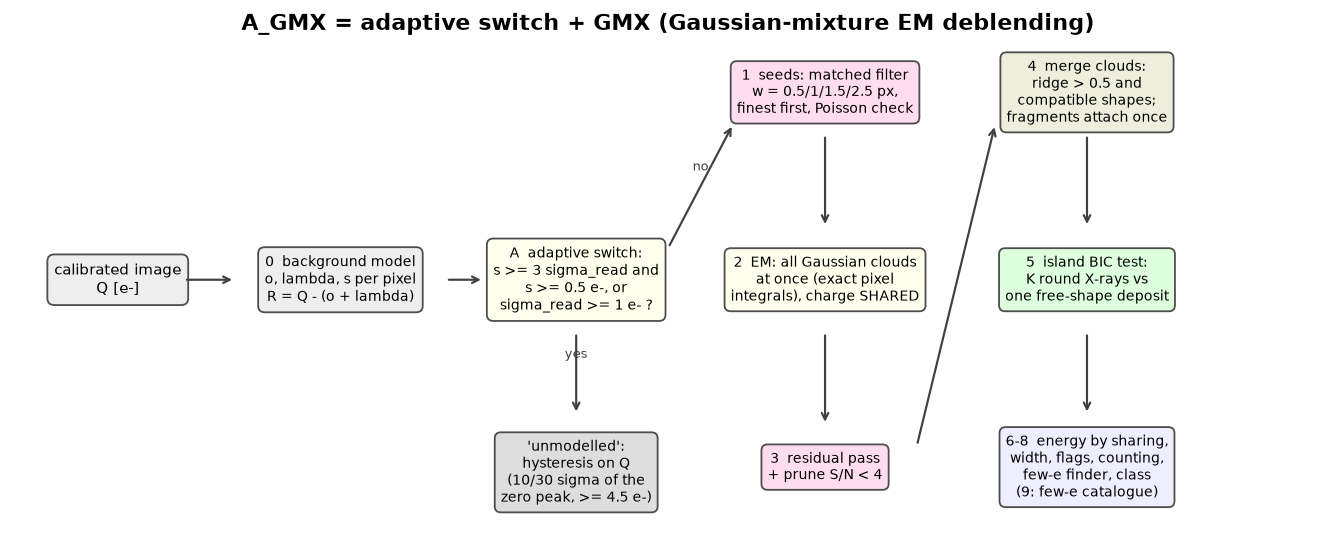
\includegraphics[width=0.95\textwidth]{figures_current/fig00_flowchart.png}
\caption{The steps of \AGMX.}
\end{figure}

\subsection*{0. Background}
\begin{itemize}
\item \textbf{Row fit.} Per row, the pixels away from clusters are fitted with the comb
$P(Q)=\sum_n\mathrm{Pois}(n;\lambda)\,\N(Q;o+n,s^2)$. Fast path: the comb phase
$z=\langle e^{2\pi iQ}\rangle$ gives $o=\arg z/2\pi$ and $s=\sqrt{-\ln|z|/2\pi^2}$, and $\lambda$ comes from the
rounded counts. A row counts as resolved only if $|z|>\max(e^{-2\pi^2\,0.45^2},\,4/\sqrt N)$, i.e.\ above the noise
floor $\sqrt{\pi/4N}$ of $N$ unresolved pixels.
\item \textbf{Unresolved rows} (comb washed out, e.g.\ by a charge sheet) take $o,\lambda,s$ from the nearest resolved
rows when at least $\max(10,\,5\,\%)$ of the rows are resolved. Otherwise a pooled comb likelihood is fitted over
groups of rows.
\item \textbf{Rounding correction.} On fast-path rows, noise above $+0.5$\,\el{} is counted as an electron:
$\lambda\leftarrow(\lambda-p)/(1-2p)$ with $p=\Phi^c(0.5/s)$.
\item $\lambda$ is smoothed along the rows (local-linear) and in column blocks, with floor $\lambda\ge10^{-6}$.
Cluster pixels are masked by a Poisson-tail test and the fit is iterated.
\item \textbf{Hot columns.} Per column, a clipped mean of $Q-o-\lambda$ (one $5\sigma$ clip around the column median)
is compared with the median of the $\pm10$ neighbouring columns. A column whose excess $d$ is $>5\times$ its error and
$>0.05$\,\el{} gets $\lambda\leftarrow\lambda+d$, so the mean, the variance and the Poisson tests all include it.
Nothing is flagged if more than 10\,\% of the columns would be (a charge sheet, not hot columns).
\item \textbf{Read noise} $\sigma_\mathrm{read}$: $1.4826\times$ the MAD of the pixels with $|Q|<0.5$\,\el. If that
exceeds 0.3\,\el, it is $\max(\text{itself},\ \text{MAD of all active pixels})$.
\end{itemize}


\begin{figure}[H]\centering
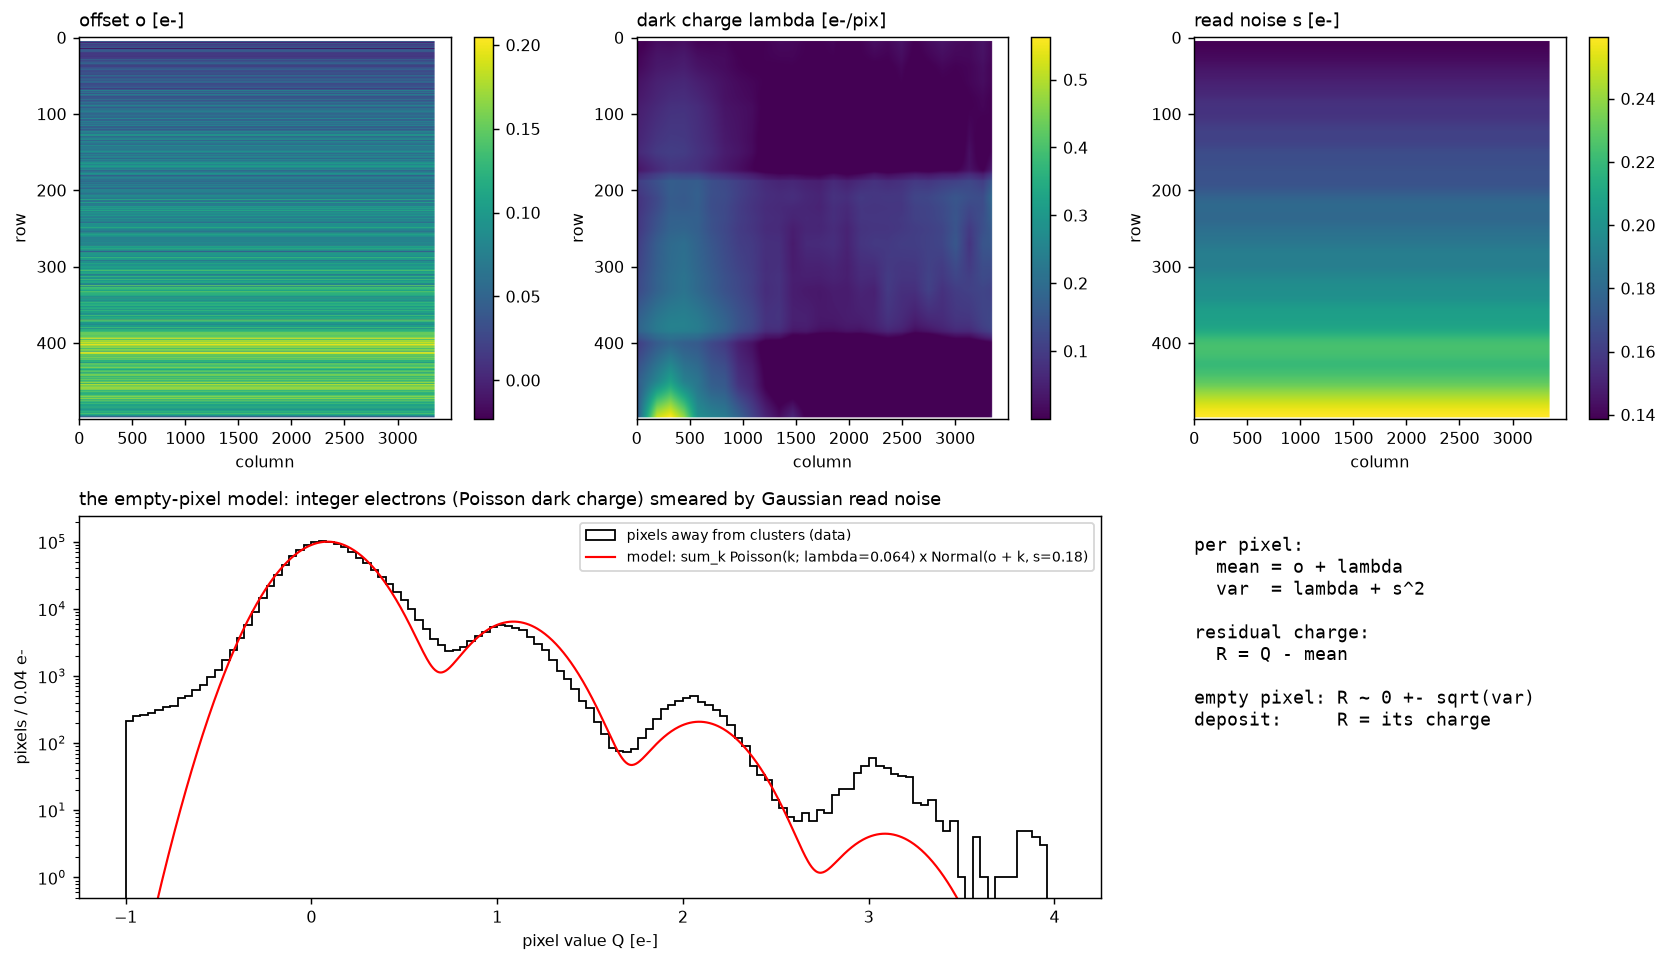
\includegraphics[width=0.95\textwidth]{figures_current/fig02_background.png}
\caption{Step 0 on the test image. Top: the fitted offset, dark-charge and read-noise maps. Bottom: the pixels away from clusters and the comb model, i.e.\ integer electrons smeared by read noise. The model curve uses the image's median $\lambda$ and $s$; the fit itself is per row, which is why the data's 2- and 3-\el{} peaks lie above a single-$\lambda$ curve.}
\end{figure}
\subsection*{A. Switch}
The image is ``unmodelled'' when $\big(s\ge0.5\,\el\text{ and }s\ge3\sigma_\mathrm{read}\big)$ or
$\sigma_\mathrm{read}\ge1$\,\el{}, where $s$ is the median of the fitted $s_p$. It is then clustered on $Q$ by
hysteresis with $\sigma_z$, the zero-peak MAD:
\begin{itemize}
\item pixels $>\max(10\sigma_z,\,4.5\,\el)$ that touch (8-connected) form a cluster;
\item it is kept if a pixel is $>\max(30\sigma_z,\,9.5\,\el)$;
\item $E=\sum Q_p$.
\end{itemize}
Otherwise GMX (steps 1--8) runs on the whole image. Every cluster also reports the event occupancy of its
$31\times31$-px neighbourhood (``crowded'' if $\ge0.3$); this is information only.

\subsection*{1. Seeds}
\begin{itemize}
\item \textbf{Matched filter} at widths $w\in\{0.5,1,1.5,2.5\}$\,px:
$T_w(c)=\sum_p h_w(p-c)R_p\big/\sqrt{\sum_p h_w(p-c)^2V_p}$. The weights $h_w$ are the exact pixel integrals of a
unit-charge Gaussian of width $w$ centred on the pixel centre, $h_w=f(i-c_y)f(j-c_x)$ with
$f(u)=\tfrac12[\mathrm{erf}((u+\tfrac12)/\sqrt2w)-\mathrm{erf}((u-\tfrac12)/\sqrt2w)]$, on $\pm\lceil4w+1\rceil$\,px. $T_w$ is a
correctly normalised significance in Gaussian sigmas. It is the optimal linear detector only for uniform noise; where $V_p$ varies
the optimal filter would also weight by $1/V_p$ (small loss of sensitivity at hot columns and gradients, no change in the
false-alarm rate), and at very low dark charge the Poisson-optimal filter of Ofek \& Zackay (2018) would be slightly better ---
hence the exact Poisson check below.
\item \textbf{Seeds} are local maxima ($5\times5$) with $T_w>5$, taken finest scale first. A coarser maximum is kept
only if no finer seed lies within $\max(2,1.5w)$\,px.
\item \textbf{Poisson check} (each seed): on the $3\times3$ or the $5\times5$ box, with $S=\sum(Q-o)$,
$\Lambda=\sum\lambda$ and $\sigma_\mathrm{b}=\sqrt{\sum s^2}$, require
$P\big(\mathrm{Pois}(\Lambda)\ge\lfloor S-2\sigma_\mathrm{b}+0.5\rfloor\big)<\Phi^c(5)$. On counting CCDs $\lambda$ is
the detection dark charge (step 7).
\item \textbf{Initial cloud:} centre = the seed pixel, $\Sigma=w^2\mathbf 1$,
$A_0=\max\!\big(R_\mathrm{seed}\,2\pi(w^2+\tfrac1{12}),\,1\big)$.
\end{itemize}


\begin{figure}[H]\centering
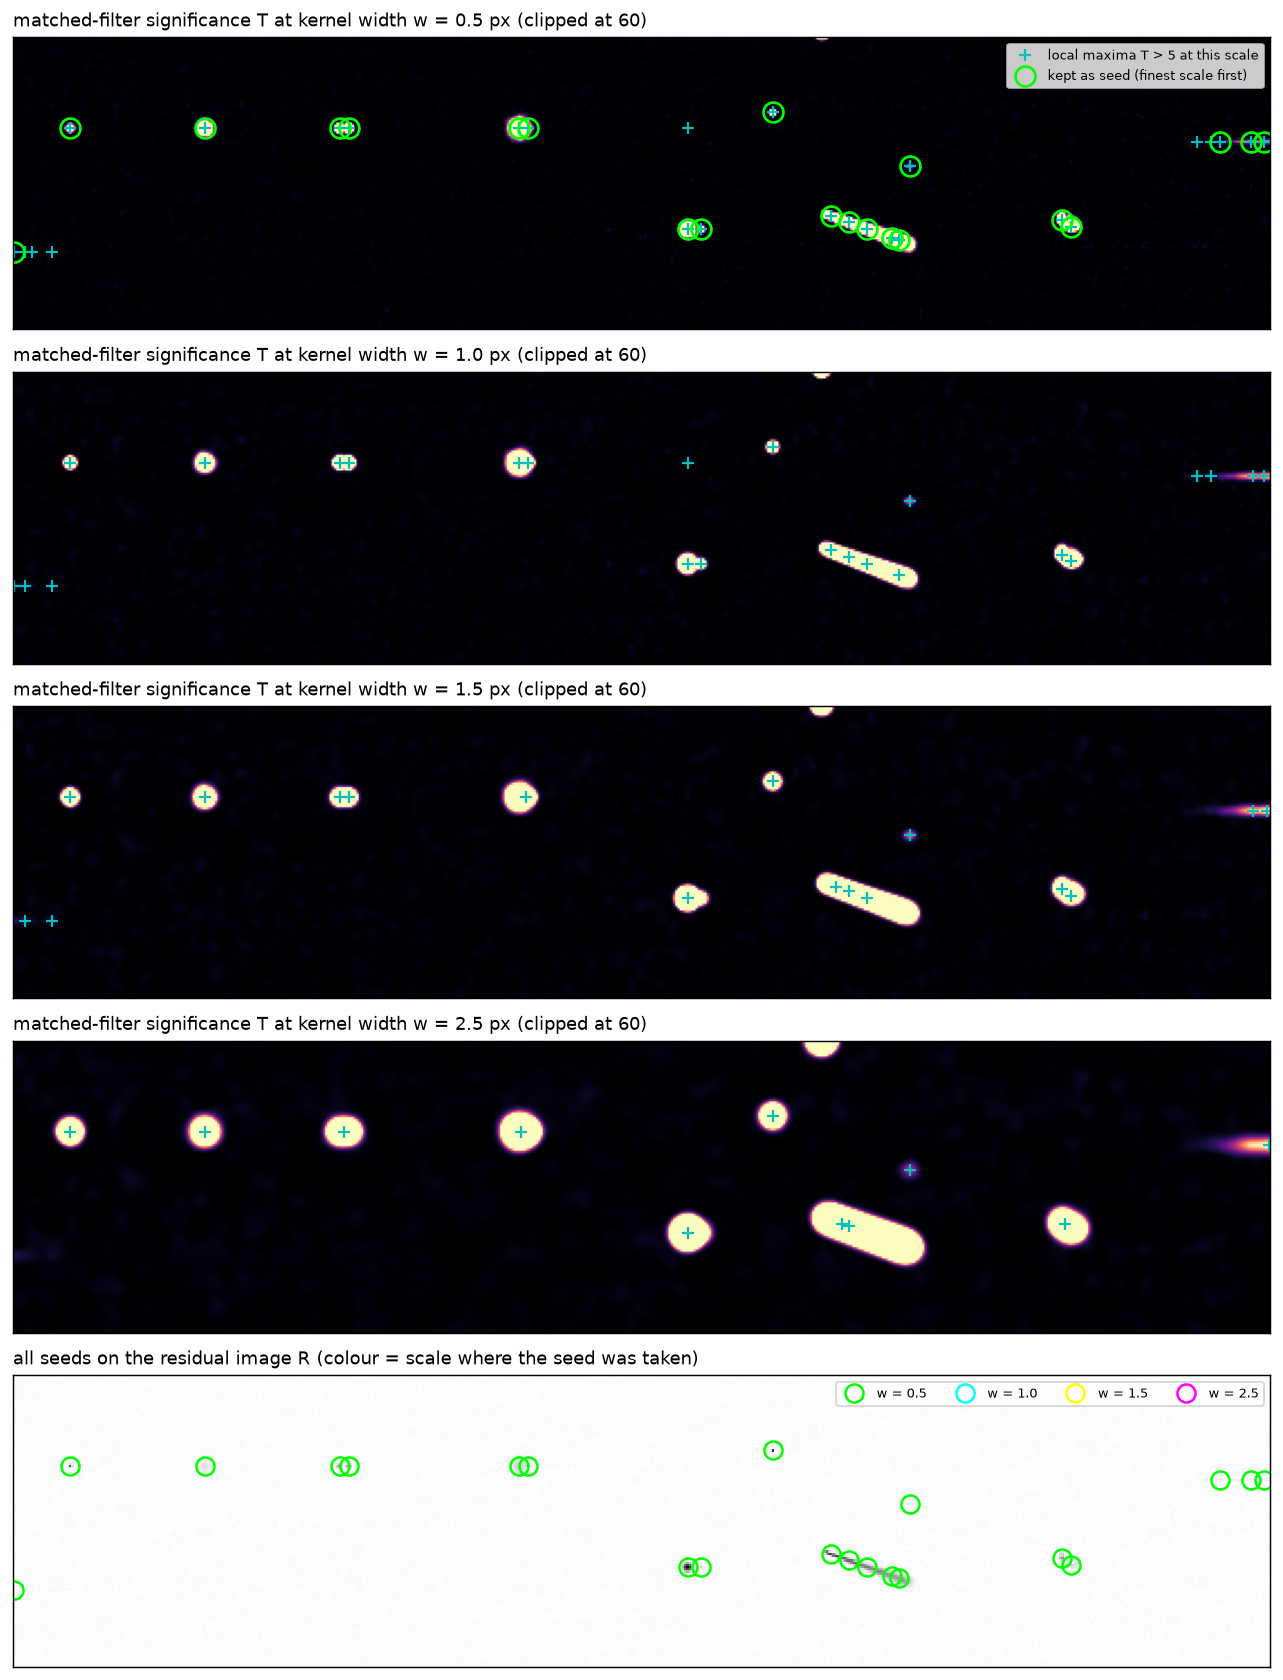
\includegraphics[width=0.82\textwidth]{figures_current/fig03_matched_filter_seeds.png}
\caption{Step 1. The matched-filter significance $T_w$ at the four widths, with the local maxima (+) and the seeds kept (circles); bottom: all seeds on $R$. Finest scale first: the 4-px pair and the sharp X-ray on the diffuse one get two seeds each, the muon and the worm several.}
\end{figure}

\begin{figure}[H]\centering
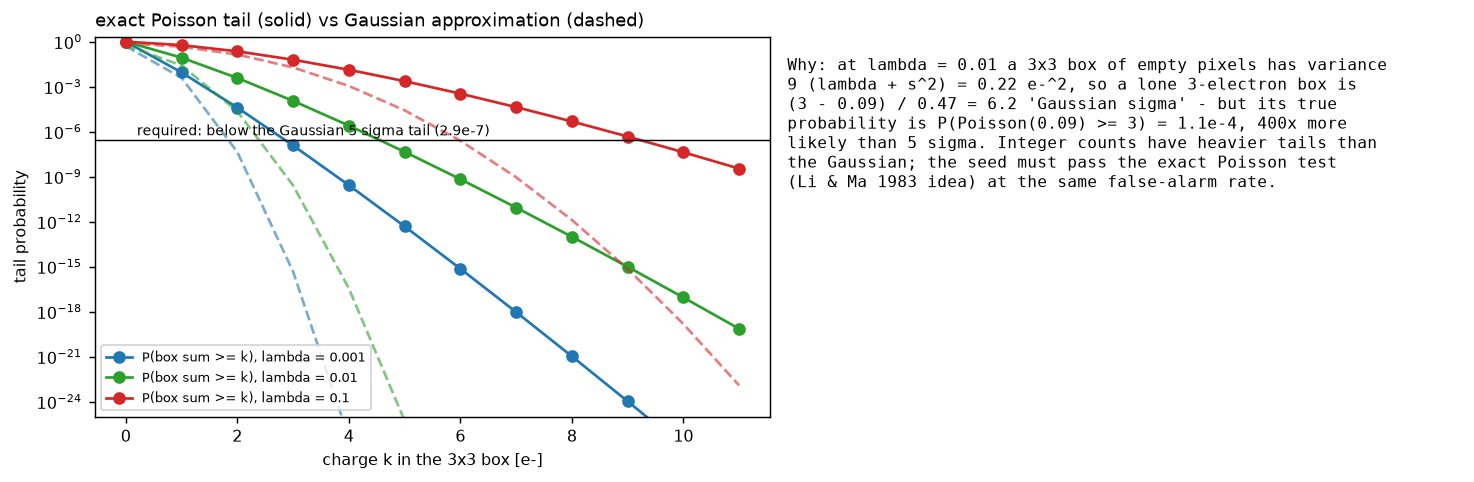
\includegraphics[width=0.9\textwidth]{figures_current/fig04_poisson_check.png}
\caption{The Poisson check: tail probability of a $3\times3$ box's charge from dark charge alone, exact (solid) versus the Gaussian approximation (dashed). At low dark charge the Gaussian is far too optimistic, so every seed must also pass the exact test at the $5\sigma$ false-alarm rate (line).}
\end{figure}
\subsection*{2. Mixture fit (EM)}
\begin{itemize}
\item \textbf{Model:} $M_p=\sum_kg_k(p)$. For a cloud with correlation $|\rho|<0.5$ (every X-ray), $g_k(p)$ is the
exact pixel integral
\[g_k(p)=A_k\big[\Phi(\tfrac{i+\frac12-\mu_y}{\sigma_y})-\Phi(\tfrac{i-\frac12-\mu_y}{\sigma_y})\big]
\big[\Phi(\tfrac{j+\frac12-\mu_x}{\sigma_x})-\Phi(\tfrac{j-\frac12-\mu_x}{\sigma_x})\big].\]
Strongly correlated clouds (pieces of tilted tracks) use $A_k\,\N(\mathbf x_p;\bm\mu_k,\Sigma_k+\tfrac1{12}\mathbf 1)$.
A cloud is evaluated within its $4\sigma$ ellipse (radius 2--16\,px).
\item \textbf{E-step:} $r_{pk}=g_k(p)/(M_p+\varepsilon_p)$, with the ``unexplained'' level $\varepsilon_p=\sqrt{V_p}$,
so noise pixels far from every cloud belong to none.
\item \textbf{M-step:} with $w_{pk}=r_{pk}R^+_p$ (cloud $k$'s share of pixel $p$, at integer coordinates $(i_p,j_p)$):
$A_k=\sum_pw_{pk}$; share moments $\bar y_k=\sum_pw_{pk}i_p/A_k$, $v^{yy}_k=\sum_pw_{pk}(i_p-\bar y_k)^2/A_k$ (likewise $x$ and
$v^{xy}_k$). These are moments of the \emph{pixelised} cloud, so for $|\rho|<0.5$ they are inverted per axis through the
pixelised-Gaussian functions $\mathcal M(\delta,\sigma^2)=\sum_ii\,\pi_i$ and $\mathcal V(\sigma^2,\delta)=\sum_i(i-\mathcal M)^2\pi_i$
($\pi_i$ the pixel integrals): $\sigma_{yy}=\mathcal V^{-1}(v^{yy}\,|\,\mathrm{frac}(\mu_y^\mathrm{old}))$, then
$\mu_y=\lfloor\bar y\rceil+\mathcal M^{-1}(\bar y-\lfloor\bar y\rceil\,|\,\sigma_{yy})$ (tabulated once, linear interpolation);
$\sigma_{xy}=v^{xy}$. For $|\rho|\ge0.5$: $\bm\mu=(\bar y,\bar x)$, $\Sigma=v-\tfrac1{12}\mathbf 1$ on the diagonal.
\item \textbf{Safeguards:} variances in $[0.02,25]$\,px$^2$, $|\sigma_{xy}|\le0.95\sqrt{\sigma_{yy}\sigma_{xx}}$,
centre step $\le1.5$\,px per iteration; clouds with $A<10^{-3}$\,\el{} are removed. 30 iterations, fixed (running
to convergence gave no consistent gain). Compiled with numba; \code{AGMX\_NUMBA=0} gives the identical numpy
version.
\end{itemize}


\begin{figure}[H]\centering
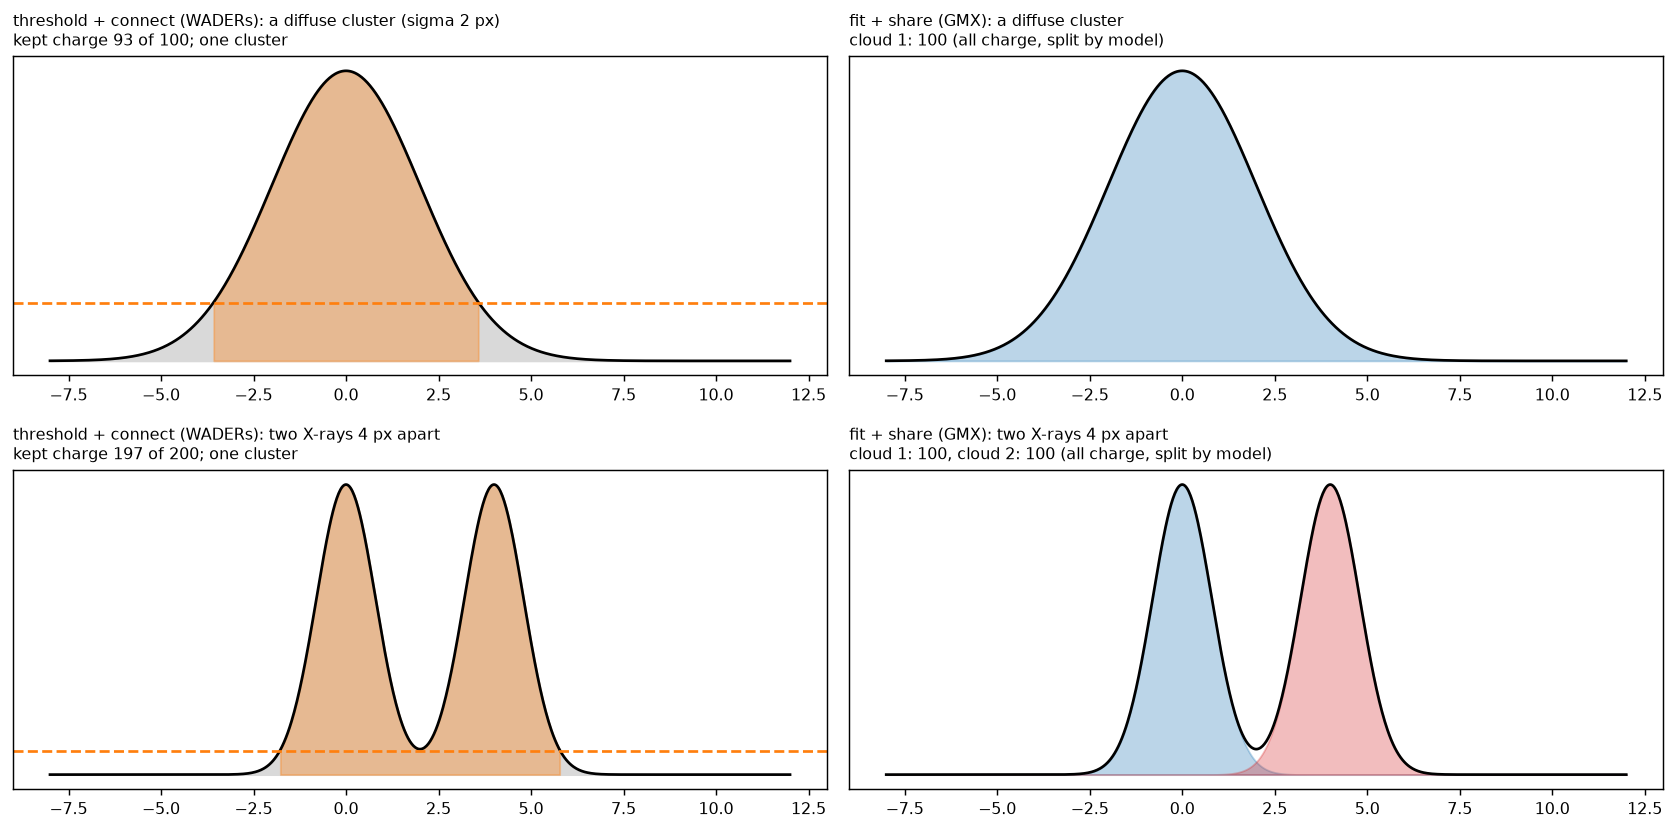
\includegraphics[width=0.85\textwidth]{figures_current/fig12_threshold_vs_sharing.png}
\caption{Why the image is fitted and shared rather than thresholded (one dimension). Left, threshold + connect: the tails of a diffuse cluster are lost and two X-rays 4\,px apart become one cluster. Right, fit + share: every electron is kept and the overlap is split in proportion to each cloud's prediction.}
\end{figure}

\begin{figure}[H]\centering
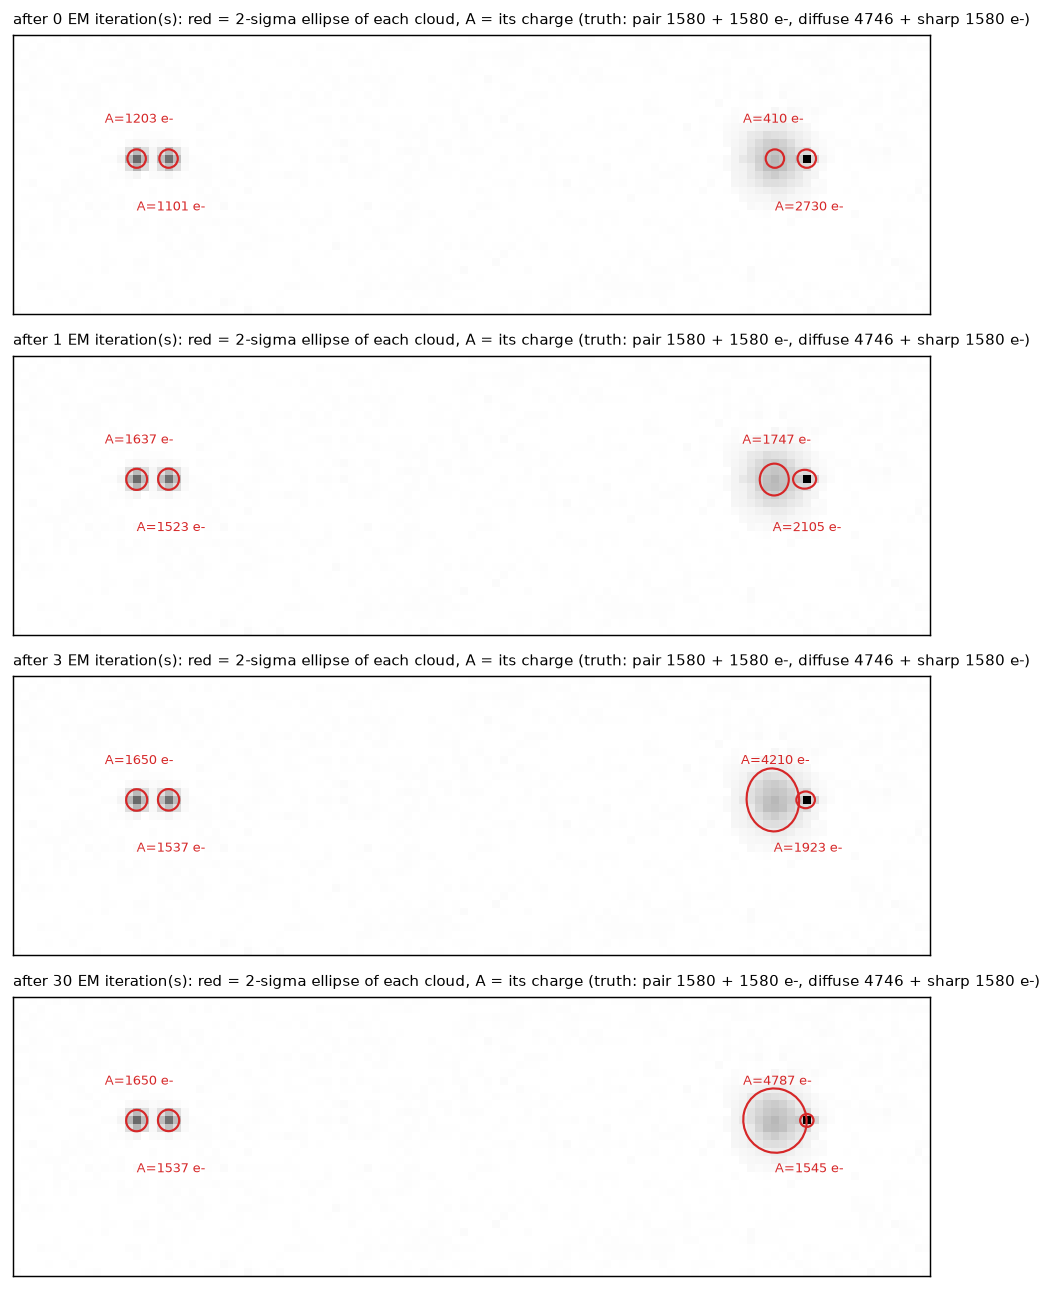
\includegraphics[width=0.75\textwidth]{figures_current/fig05_em_evolution.png}
\caption{Step 2. EM on the 4-px pair (left) and on the sharp X-ray on a diffuse one (right): the $2\sigma$ ellipses and charges $A$ after 0, 1, 3 and 30 iterations. The diffuse cloud grows to its width, the sharp one shrinks onto its pixel; final charges 1650 + 1537\,\el{} and 4787 + 1545\,\el{} (nominal 1580 + 1580 and 4746 + 1580; the injected numbers are Poisson draws).}
\end{figure}

\begin{figure}[H]\centering
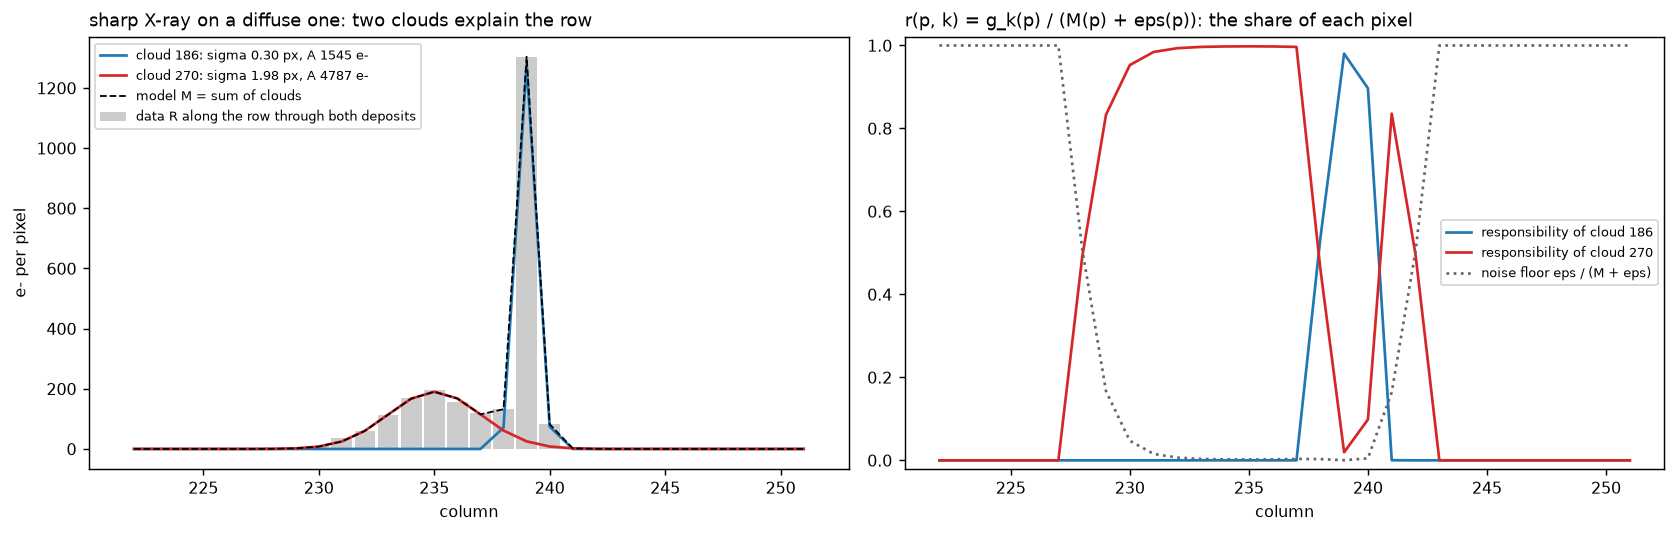
\includegraphics[width=0.95\textwidth]{figures_current/fig06_responsibilities.png}
\caption{Charge sharing in the row through the sharp X-ray on the diffuse one. Left: data, the two clouds ($\sigma$ 0.30 and 1.98\,px) and their sum. Right: the responsibilities $r_{pk}$, i.e.\ each pixel's share per cloud; far from both clouds the noise share is 1, so those pixels go to no cloud.}
\end{figure}
\subsection*{3. Residual pass and pruning}
\begin{itemize}
\item \textbf{Residual pass.} The matched filter is run on $R-M$ with variance $V+M$ at $w=0.5,1$. Local maxima
($3\times3$) with $T>5$, passing the Poisson check (counting CCDs) and more than 1\,px from every cloud, become new
clouds. Then 15 EM iterations.
\item \textbf{Pruning.} Clouds with $\mathrm{S/N}_k=A_k\sqrt{\sum_p\pi_k(p)^2/(V_p+M_p-g_k(p))}<4$ are dropped, where
$\pi_k=g_k/A_k$. Then 5 EM iterations.
\end{itemize}


\begin{figure}[H]\centering
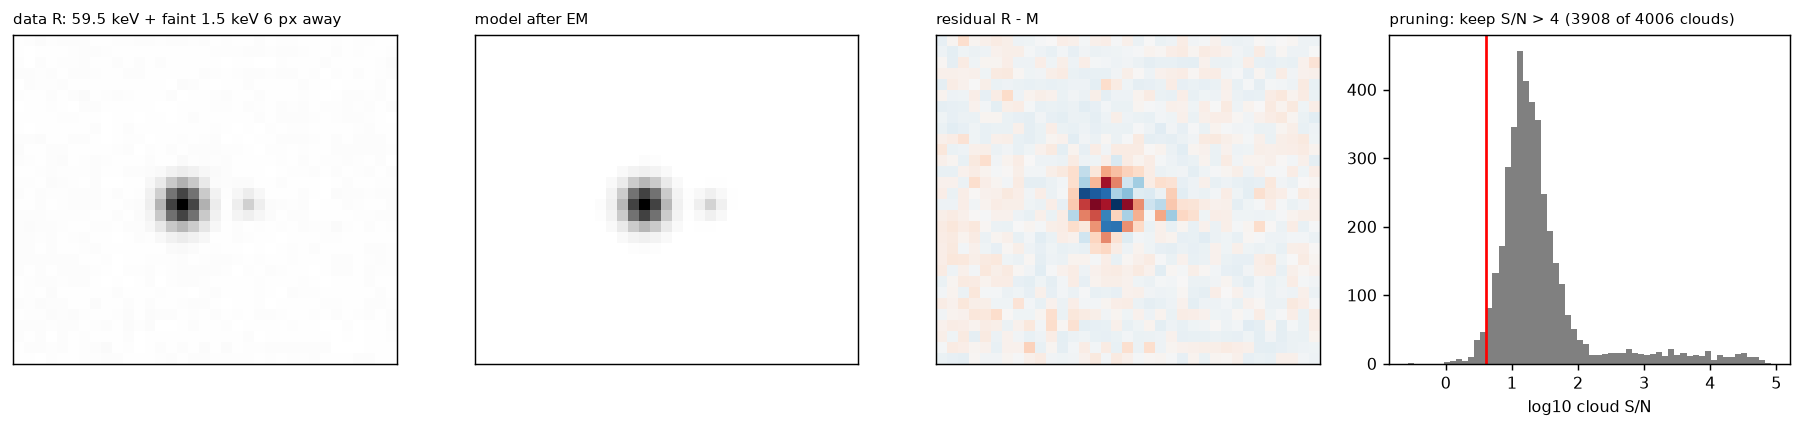
\includegraphics[width=0.95\textwidth]{figures_current/fig07_residual_pruning.png}
\caption{Step 3. A 59.5-keV X-ray with a faint 1.5-keV X-ray 6\,px away: data, model, residual. Right: the S/N of all clouds of the image with the cut S/N\,$>4$ (3908 of 4006 clouds kept).}
\end{figure}
\subsection*{4. Grouping clouds into deposits}
Every pair closer than $3.5(\bar\sigma_i+\bar\sigma_j)+1$\,px is tested ($\bar\sigma$: geometric-mean width,
$\le16$\,px).
\begin{itemize}
\item \textbf{Ridge test:} $\rho_{ij}=\min_tf(t)/\min(f(0),f(1))>0.5$, where $f$ is the two-cloud density along the
line joining the centres (17 points).
\item \textbf{Shape test}, one of: width ratio $<1.6$; a track (one cloud has axis ratio $>1.4$ and its long axis is
within $|\cos|>0.8$ of the joining line); or the narrower cloud is not a local maximum of $f$ (a shoulder).
\item \textbf{Fragments.} A cloud below 50\,\el{} \emph{and} below 10\,\% of its brightest merge partner links only
to that partner, so it cannot join an X-ray to a neighbouring large deposit.
\end{itemize}
Clusters are the connected components of the links.


\begin{figure}[H]\centering
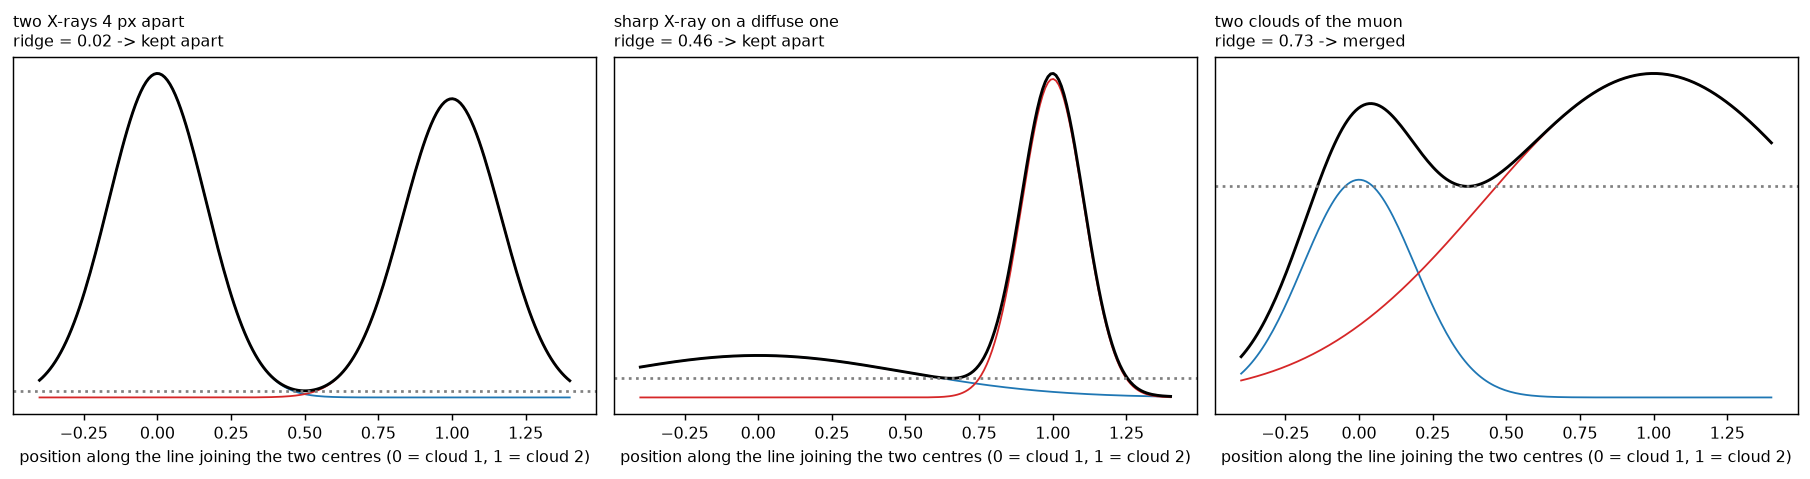
\includegraphics[width=0.95\textwidth]{figures_current/fig08_ridge_test.png}
\caption{Step 4, ridge test: the two-cloud density along the line between the centres. Two X-rays 4\,px apart: deep valley ($\rho=0.02$), kept apart. A sharp X-ray on a diffuse one: $\rho=0.46<0.5$, kept apart (it is also a maximum of its own with a very different width). Two clouds of the muon: $\rho=0.73$, merged.}
\end{figure}
\subsection*{5. Island test (tracks versus several X-rays)}
Islands are 8-connected regions above the Poisson-tail threshold of the dark charge ($\alpha=0.01$), of at most
4000\,px. An island holding $K\ge2$ clusters is refitted on its pixels (+2 rings) under two hypotheses:
\begin{itemize}
\item $K$ round Gaussians (4 parameters each);
\item the free clouds already fitted (6 parameters each, $n_c$ clouds).
\end{itemize}
They are compared by
\[\Delta\mathrm{BIC}=\chi^2_\mathrm{round}+4K\ln n-\chi^2_\mathrm{free}-6n_c\ln n,\qquad
\chi^2=\sum_p\frac{(R_p-M_p)^2}{V_p+R^+_p+(0.05R_p)^2}.\]
If $\Delta\mathrm{BIC}>100$ the whole island becomes one deposit (30 with \code{AGMX\_PIX\_EXACT=0}).


\begin{figure}[H]\centering
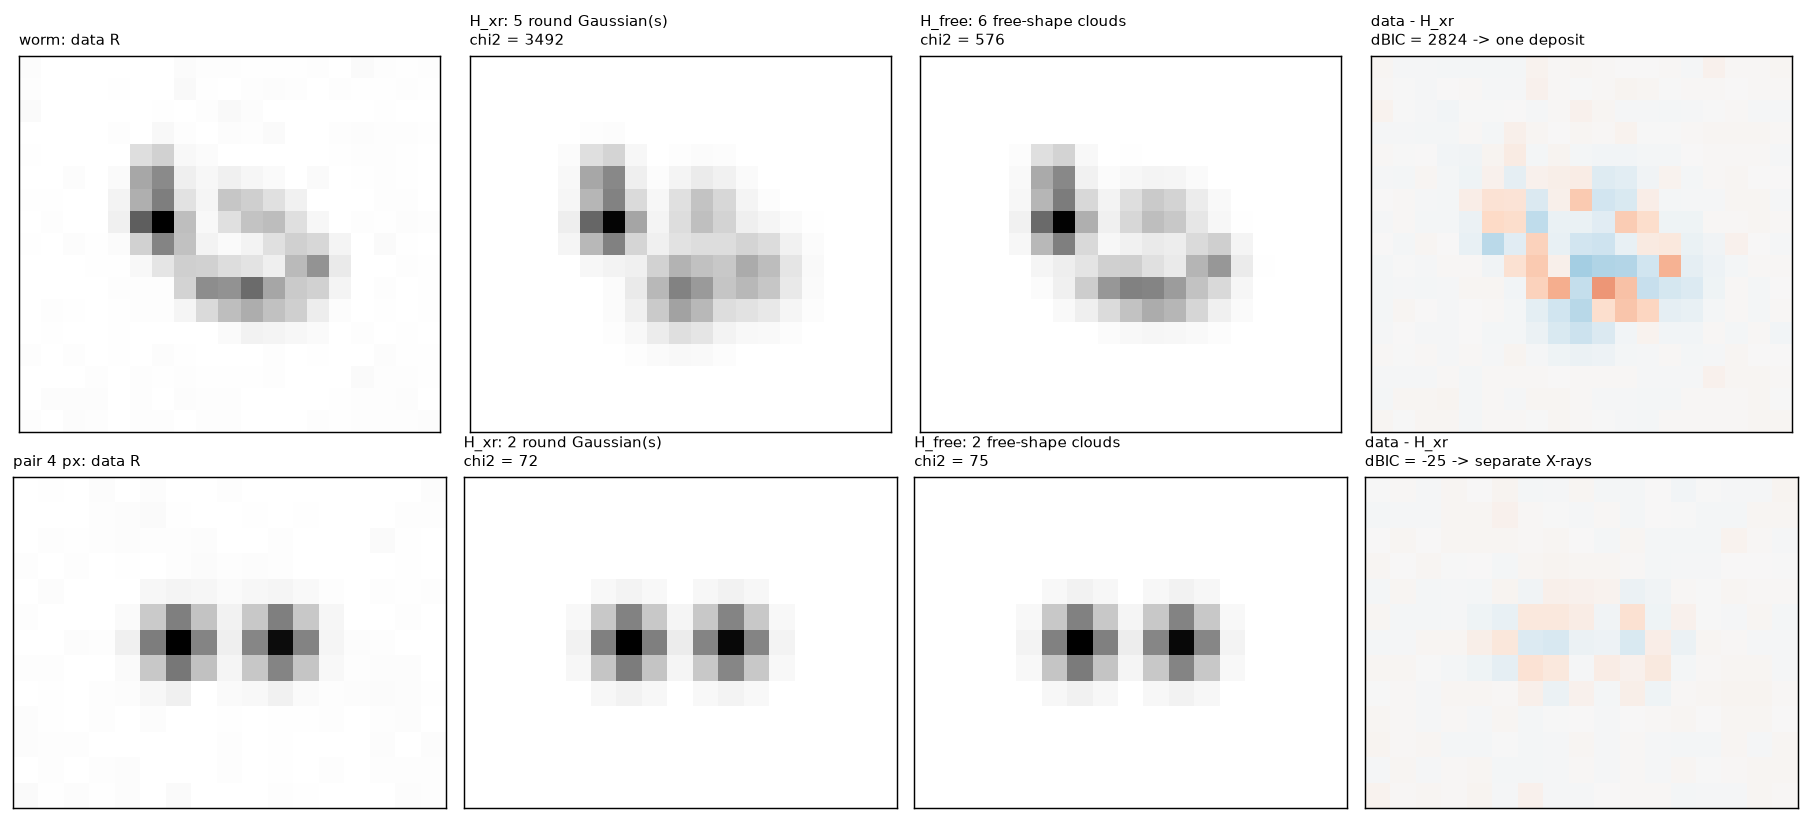
\includegraphics[width=0.95\textwidth]{figures_current/fig13_island_example.png}
\caption{Step 5. Top, the worm: 5 round Gaussians cannot follow the bent track ($\chi^2$ 3492, structured residual) and 6 free-shape clouds can ($\chi^2$ 576), so $\Delta\mathrm{BIC}=2824>100$ and the island is one deposit. Bottom, the 4-px pair: both descriptions fit equally well ($\chi^2$ 72 vs 75) and the round one has fewer parameters, so $\Delta\mathrm{BIC}=-25$ and it stays two X-rays.}
\end{figure}
\subsection*{6. Energy, width and flags}
\begin{itemize}
\item \textbf{Energy by sharing:} $E_c=\sum_p\tilde r_{pc}R_p$, with $\tilde r_{pc}=\sum_{k\in c}g_k(p)/M_p$. The
measured charge is split, never counted twice.
\item \textbf{Satellites.} A cluster with $E<1\,\%$ of a neighbour's \emph{and} $E<1$\,keV is merged into that
neighbour if its centre lies in the neighbour's domain or within $6\sigma$ (Mahalanobis) of one of its clouds
(within 20\,px).
\item \textbf{Growth.} Pixels above the $\alpha=0.01$ Poisson tail, within 3\,px of a covered pixel, connected to it
and covered by no cloud (charge-transfer trails), are added to the nearest cluster.
\item \textbf{Width:} $\sigma_{xy}^2=\tfrac12(\mathrm{var}_y+\mathrm{var}_x)-\tfrac1{12}$, the second moments of the
cluster's shared charge. A single cloud whose EM width is $<0.4$\,px reports the EM width, because the moment is
noise-dominated there.
\item \textbf{Flags}, which never change the energy:
  \begin{itemize}
  \item blend $=\sum_pM^{(c)}_pM^{(\neg c)}_p/\sum_p(M^{(c)}_p)^2$ (other clusters' charge under this one's profile);
  \item ped: the 25th percentile of $R$ in a ring 5--8\,px around the centre (a charge sheet);
  \item peakfrac: the largest cloud's share of the fitted charge;
  \item $\chi^2$: $\sum(R-M)^2/(V+M)$ per pixel over the pixels the cluster owns ($\tilde r>0.5$);
  \item sig: $E_c/\sqrt{\sum\tilde r^2V}$;
  \item edge: within 2\,px of the mask;
  \item saturated: a pixel at an ADC-limit plateau.
  \end{itemize}
\end{itemize}


\begin{figure}[H]\centering
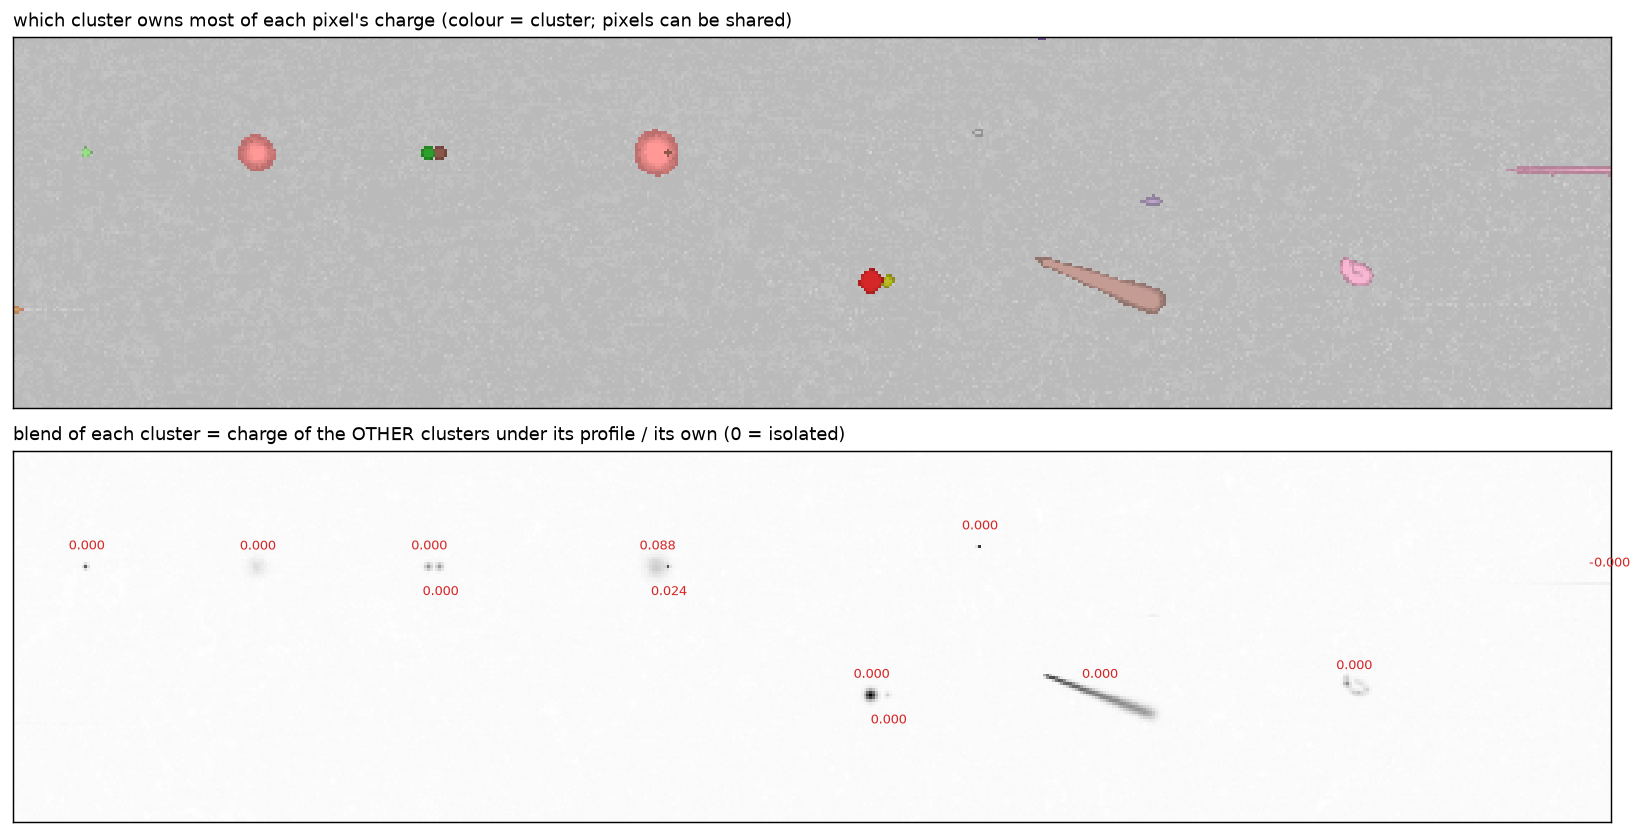
\includegraphics[width=0.95\textwidth]{figures_current/fig10_ownership_blend.png}
\caption{Step 6. Top: which cluster owns most of each pixel's charge (pixels can be shared). Bottom: the blend flag of each cluster, 0 for isolated clusters and 0.088 / 0.024 for the sharp X-ray on the diffuse one, whose profiles overlap.}
\end{figure}
\subsection*{7. Few-electron events (median $s<0.35$\,\el)}
\begin{itemize}
\item \textbf{Detection dark charge} $\lambda_\mathrm{det}$: $\lambda$ implied by the rate of \emph{isolated}
single-electron pixels (no counted pixel within 2\,px; smoothed over $\pm30$ rows; rounding miscounts included),
never below the fitted map, plus the hot-column excess.
\item \textbf{Counting energies.} A cluster below 100\,\el{} gets
$E=\sum_{\tilde r>0.5}\big(\mathrm{round}(Q-o)-\lambda\big)$; the analog value is kept as \code{E\_fit}.
\item \textbf{Counting finder.} An 8-connected group of $\le9$ pixels with $\mathrm{round}(Q-o)\ge1$, not covered by
a cluster, has statistic $T=-\sum_i\ln P(n_i\,|\,\lambda_{\mathrm{det},i},s_i)-\ln N_\mathrm{shapes}(m)$, with
$P(n|\lambda,s)=\sum_k\mathrm{Pois}(k;\lambda)\big[\Phi(\tfrac{n+\frac12-k}{s})-\Phi(\tfrac{n-\frac12-k}{s})\big]$.
The group is kept when $T$ exceeds the value exceeded by 0.08 groups per Mpix in 10--50 blank images simulated
from the image's own $\lambda_\mathrm{det},s$ (fixed seed). The analytic bound $\ln(N_\mathrm{pix}/F)$ is used only
if the blanks have too few groups. Class ``low-E''.
\end{itemize}


\begin{figure}[H]\centering
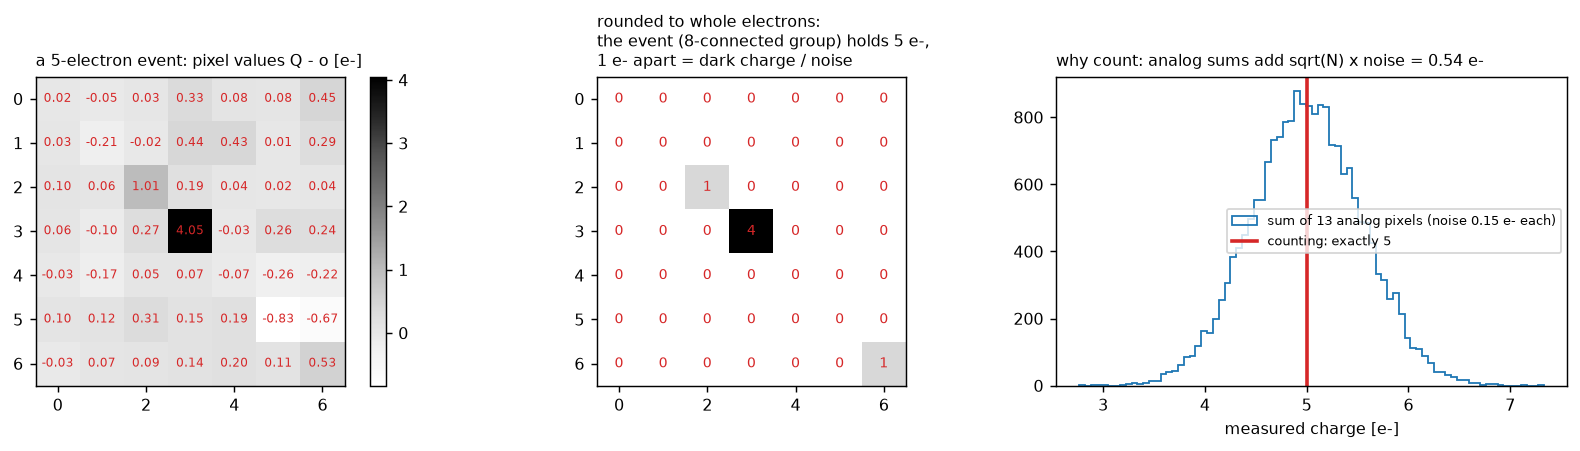
\includegraphics[width=0.95\textwidth]{figures_current/fig11_counting.png}
\caption{Step 7. A 5-electron event: analog pixel values; the same rounded to whole electrons (the event's 8-connected group holds 5\,\el; the 1\,\el{} in the corner is a separate dark-charge or noise pixel, a group of its own); and the spread an analog sum over 13 pixels would have (0.54\,\el) against the exact count.}
\end{figure}
\subsection*{8. Classes}
\begin{itemize}
\item \textbf{low-E:} $E<0.5$\,keV.
\item \textbf{x-ray / x-ray diffuse:} one round cloud or extent $<6$\,px; diffuse if $\sigma_{xy}\ge1$.
\item \textbf{alpha:} $>1$\,MeV.
\item \textbf{artifact-row / -column:} thin, straight and aligned with a row or column.
\item \textbf{muon:} straight skeleton ($\ge10$\,px, scatter of the cloud centres $<1$\,px and $<6\,\%$ of the
length) \emph{and} $\ge2.5$\,keV per projected pixel; a straight track below that rate is ``extended''.
\item \textbf{worm:} everything else extended.
\end{itemize}

\subsection*{9. After A\_GMX: the few-electron candidate catalogue}
For counting CCDs, written to \code{fe\_candidates/*\_fe\_candidates.csv} and \code{.json} (off with
\code{--no-fe-candidates}):
\begin{itemize}
\item \textbf{Candidates:} every group of 2--20 counted electrons ($\le9$\,px), with $T$, $n_\mathrm{exp}$ (expected
dark-charge groups per image at least as unlikely; simulated blanks of the image's own occupancy-based $\lambda$) and
$p_\mathrm{image}=1-e^{-n_\mathrm{exp}}$.
\item \textbf{Mask flags:} halo ($5\sqrt{E/\mathrm{keV}}$\,px, 5--60) around clusters, row/column trails (50\,px,
$E>1$\,keV), hot columns, edge (5\,px), overlap with a cluster.
\item \textbf{Per image:} observed and expected clean counts per class (charge, pixels).
\end{itemize}
Nothing is removed; it is the input for a rare-event analysis.

\paragraph{Recommended selection for X-ray lines:} $\sigma_{xy}<0.7$ (Am-241) or $<1$ (front-side Fe-55), blend
$<0.02$, ped $<10$\,\el/pix, not edge.

\paragraph{Switches} (environment): \code{AGMX\_PIX\_EXACT=0} (Gaussian-at-centre model, BIC margin 30, no fragment
rule), \code{AGMX\_PHYS\_FIXES=0} (behaviour before the 25--26 October audit), \code{AGMX\_NUMBA=0},
\code{AGMX\_FE\_CANDIDATES=0}.

%======================================================================================================
\section{Comparison with WADERs}

WADERs: panaSKImg's ClusterFinder, i.e.\ hysteresis with pixel $>10\sigma$ and seed $>30\sigma$ of the pedestal,
$E=\sum$ core pixels. The tests below use the same injected objects and the same images for both methods.
\textbf{Code versions:} the crowded-CCD fit is from the current code (26 October). The wide, Fe-55-width, track and
few-electron tests were run on the code of 25 October, before the physics audit and the exact pixel integrals. On a
subset (80 image-CCDs) the current code changes front-side K$\alpha$ by $-0.2$\,eV (median) and resolves more pairs
(Fe-55 0.907$\to$0.941, Am-241 0.607$\to$0.655). A full rerun of those tests is pending.

\begin{table}[H]\centering\small
\begin{tabularx}{\textwidth}{>{\raggedright\arraybackslash}X ccc}
\toprule
 & WADERs & \AGMX & code \\
\midrule
\multicolumn{4}{@{}l}{\textit{Crowded Am-241 CCD (AMtest EXT4, 29 images), constrained 10--30\,keV fit (L\'epy line ratios)}} \\
energy scale $k$ (1 = right) & 0.9840 & \textbf{1.0006} & 26 Oct \\
Np L$\beta$ / L$\gamma$ / $\gamma$\,26.3 / Ag K significance [$\sigma$] & 15.5 / 16.0 / 14.8 / 12.9 & \textbf{22.4 / 20.6 / 21.1 / 18.3} & 26 Oct \\
combined $Z$ (Np L + $\gamma$\,26.3) & 27.1 & \textbf{37.4} & 26 Oct \\
deviance / ndf & \textbf{1.74} & 2.59 & 26 Oct \\
\midrule
\multicolumn{4}{@{}l}{\textit{Fe-55 (DM09/DM10, 220 injected clusters per width and CCD; 8 CCDs)}} \\
energy of injected clusters, width $0.3\to1.8$\,px (median) & $0.997\to0.921$ & $\mathbf{1.000\to1.000}$ & 25 Oct \\
worst CCD at width 1.8\,px & 0.737 & \textbf{0.994} & 25 Oct \\
real front-side K$\alpha$ / 5.899\,keV: mean, spread over 8 CCDs & 0.9928, 1.32\,\% & \textbf{0.9969, 0.23\,\%} & 25 Oct \\
two diffuse ($\sigma$ 1.4\,px) clusters 5\,px apart resolved & 0.00 & \textbf{0.93} & 25 Oct \\
\midrule
\multicolumn{4}{@{}l}{\textit{Wide test: 878 image-CCDs, 16 data sets, injected objects}} \\
Fe-55 / muon / worm / 4-px pair success & 0.86 / 0.59 / 0.74 / 0.11 & \textbf{0.93 / 0.64 / 0.79 / 0.88} & 25 Oct \\
Fe-55 energy resolution (rms of $E/E_\mathrm{true}$) & 0.52\,\% & \textbf{0.19\,\%} & 25 Oct \\
dark charge $\ge1$\,\el/pix: Fe-55 / worm / pair & 0.55 / 0.45 / 0.07 & \textbf{0.87 / 0.74 / 0.79} & 25 Oct \\
\midrule
\multicolumn{4}{@{}l}{\textit{Injected objects in real Am-241 images (EXT1)}} \\
alpha / low-E / 3-px pair / 4-px pair & 0.90 / 0.47 / 0.00 / 0.21 & \textbf{0.94 / 0.64 / 0.75 / 0.93} & 25 Oct \\
muon / worm / hot column & 0.90 / 0.93 / \textbf{0.76} & 0.93 / 0.93 / 0.74 & 25 Oct \\
\midrule
\multicolumn{4}{@{}l}{\textit{Few-electron events (simulated, 0.15\,\el{} noise)}} \\
3-\el{} found at $10^{-3}$\,\el/pix & 0.00 & \textbf{0.85} (fakes 0.07 per 1.7\,Mpix) & 26 Oct \\
3-\el{} found at $10^{-4}$\,\el/pix & not run & \textbf{0.96} (fakes 0.30 per 1.7\,Mpix) & 26 Oct \\
\midrule
run time per image-CCD (median) & \textbf{0.01\,s} & 0.7\,s (Fe-55 0.9\,s, Am-241 62\,s) & 25/26 Oct \\
\bottomrule
\end{tabularx}
\end{table}

\begin{figure}[H]\centering
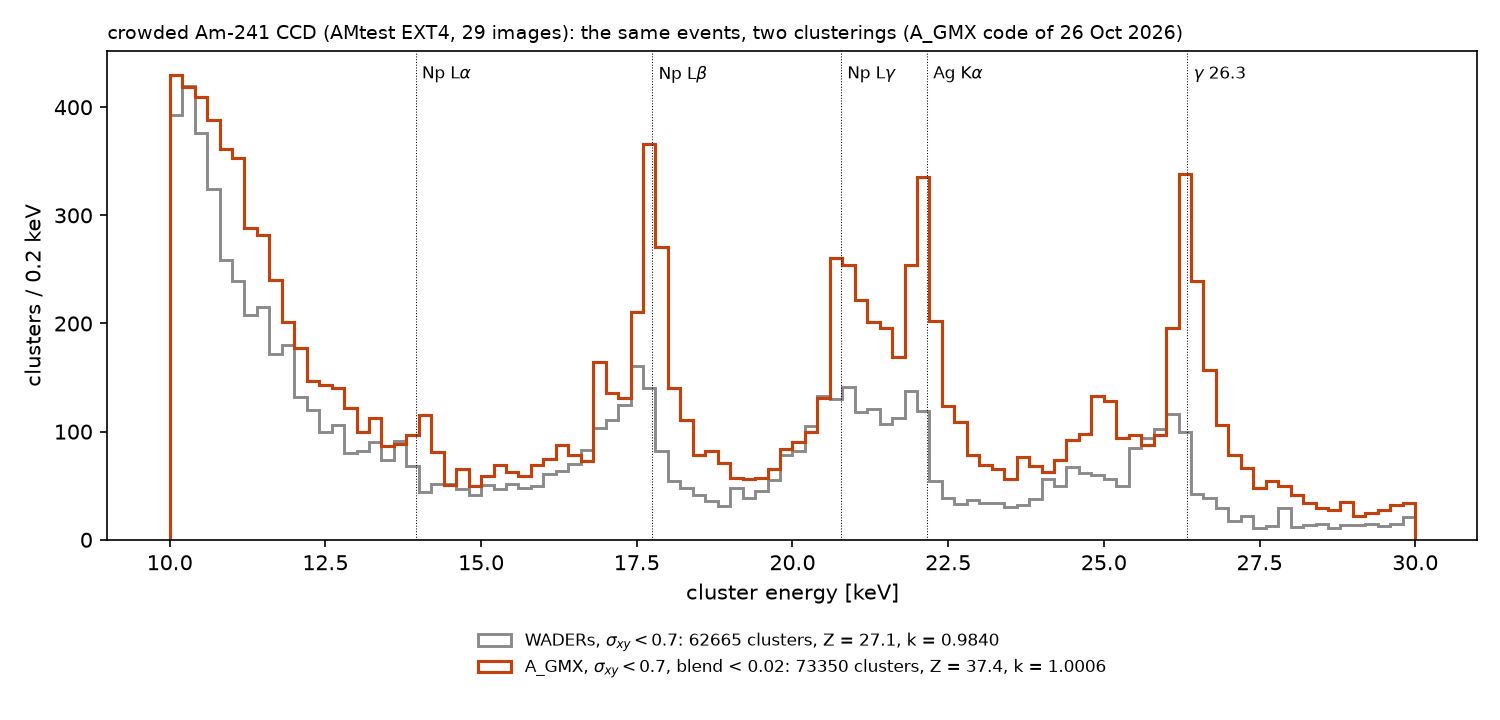
\includegraphics[width=0.92\textwidth]{figures/figC1_crowded_current.png}
\caption{The crowded CCD, current code: the same events clustered by WADERs and by \AGMX{} (blend $<0.02$). \AGMX's
lines are higher above the continuum and at the right energy ($k=1.0006$ vs 0.984). Not yet understood: its spectrum
between the lines fits worse (deviance/ndf 2.59 vs 1.74).}
\end{figure}

\begin{figure}[H]\centering
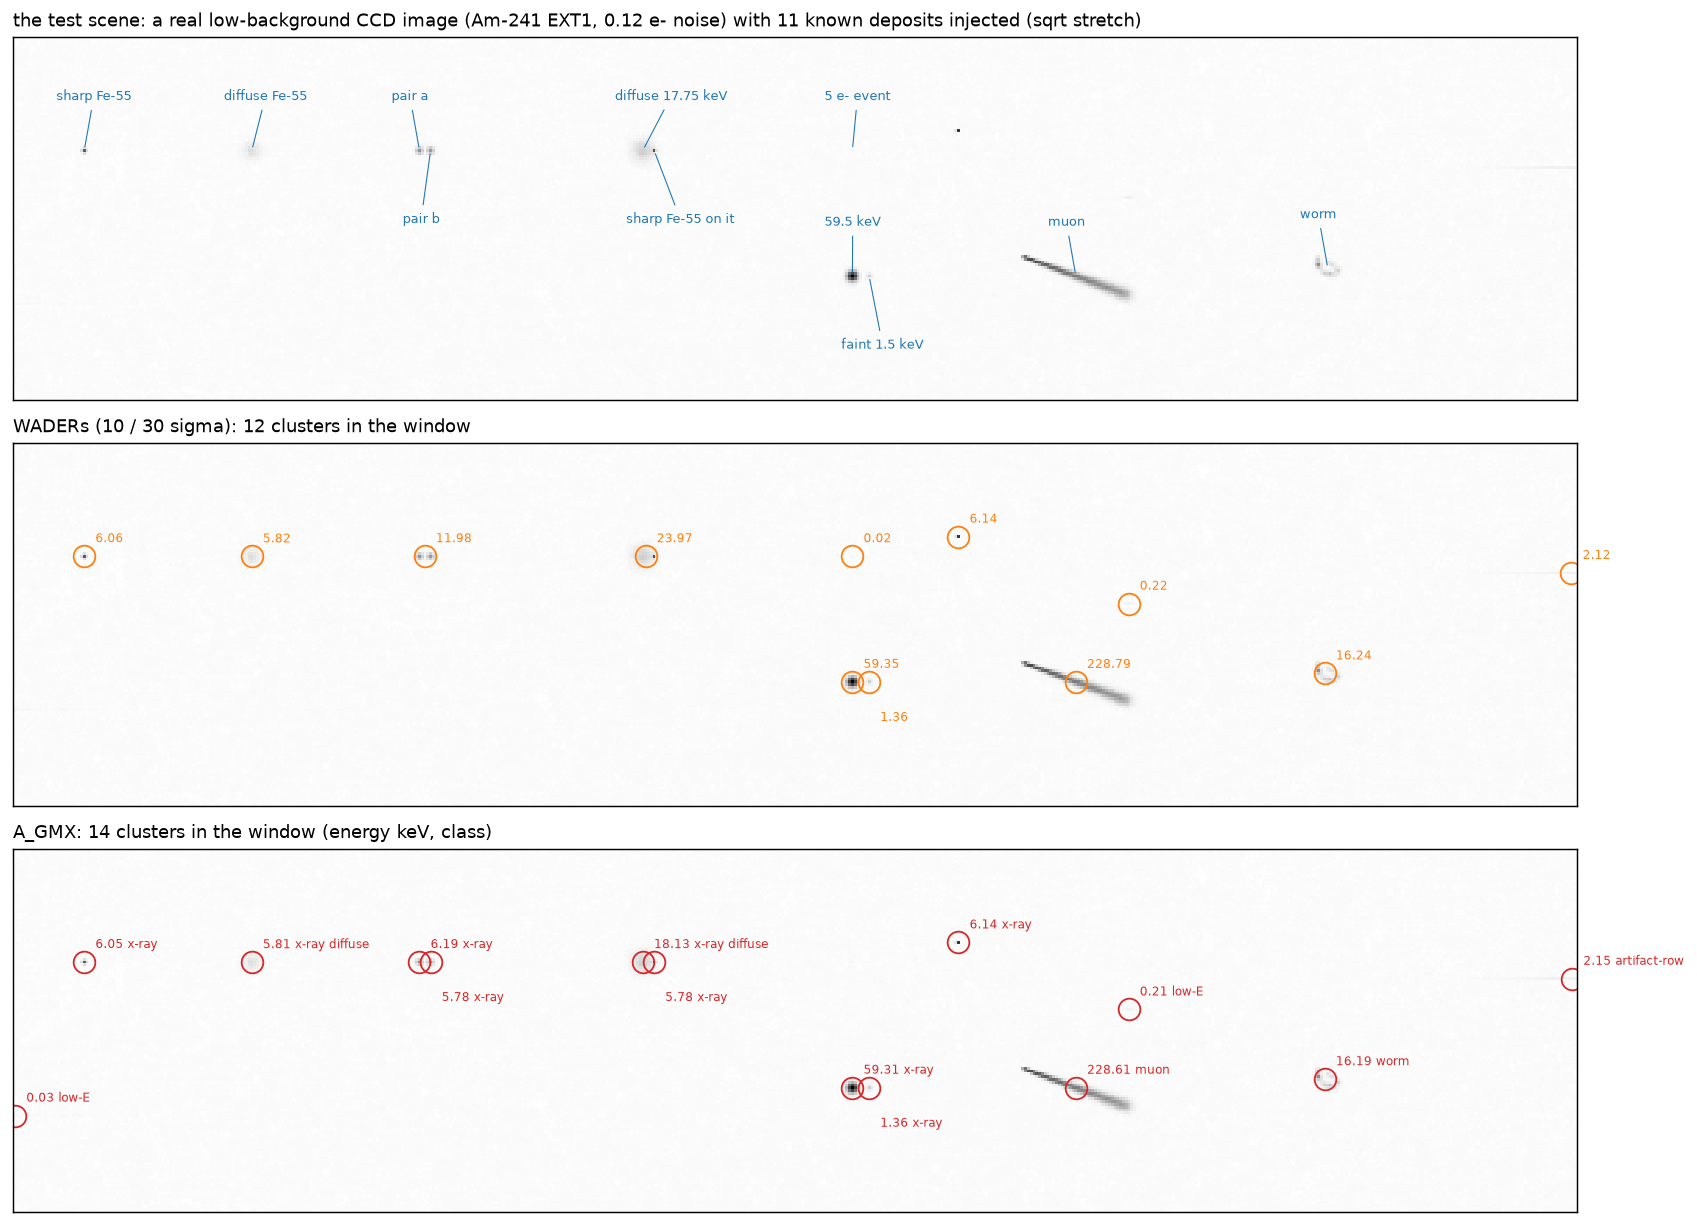
\includegraphics[width=0.92\textwidth]{figures_current/fig01_overview.png}
\caption{The test scene of section~2 (top). WADERs (middle) merges the 4-px pair into one 12-keV cluster
and the sharp X-ray on the diffuse one into one 24-keV cluster. \AGMX{} (bottom) separates both: 6.19 + 5.78\,keV (truth
6.20 + 5.77) and 18.13 + 5.78\,keV (truth 18.07 + 5.82). The 5-\el{} event (4\,\el{} in one pixel) is found by WADERs
(0.015\,keV) but not by \AGMX: at the $\sim$0.07\,\el/pix dark charge there, a group this size is not significant at
\AGMX's calibrated fake rate of 0.08 per Mpix (WADERs has no fake-rate control; figure~\ref{fig:lowe} and the table give
the rates). Current code.}\label{fig:scene}
\end{figure}

\begin{figure}[H]\centering
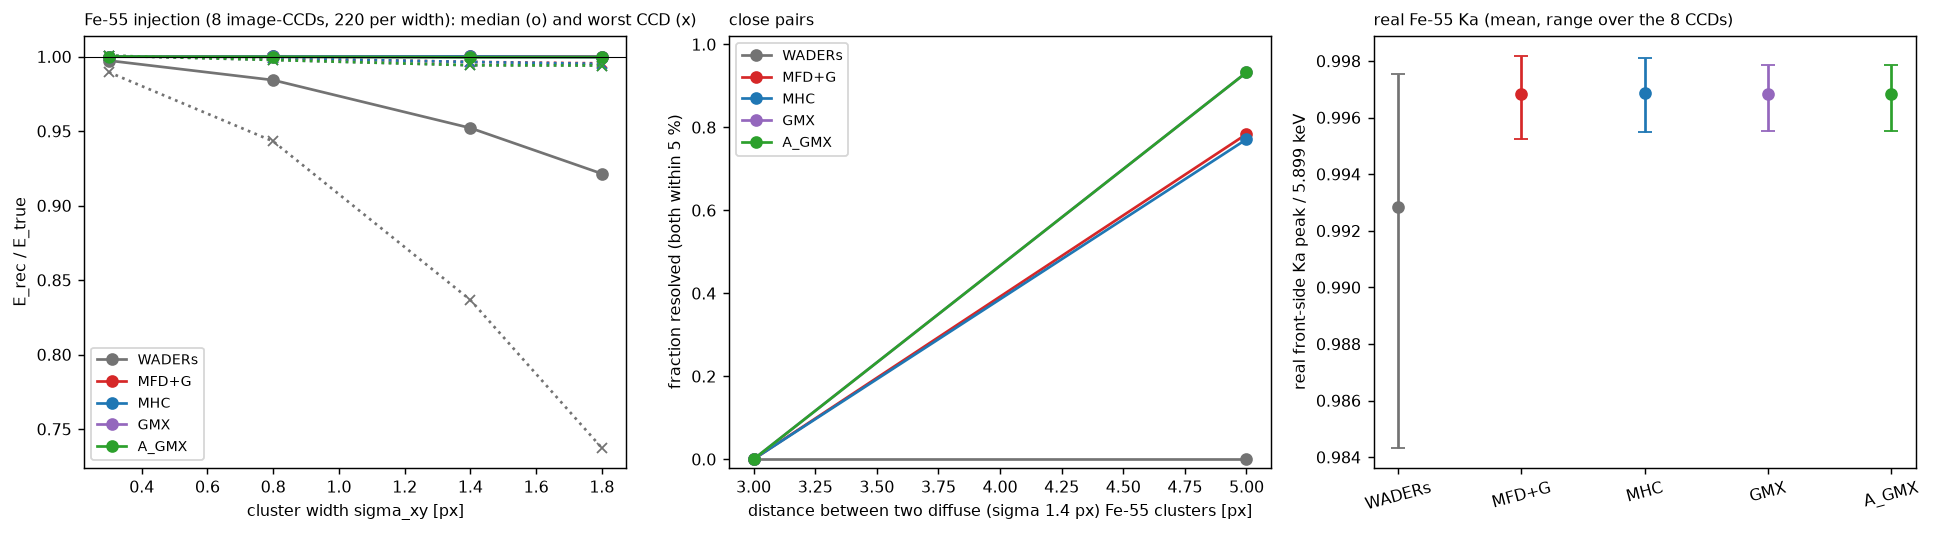
\includegraphics[width=0.92\textwidth]{figures/fig22_fe55.png}
\caption{Fe-55. Left: median (circles) and worst-CCD (crosses) $E_\mathrm{rec}/E_\mathrm{true}$ against cluster
width; WADERs' thresholds cut the tails of diffuse clusters. Middle: diffuse pairs resolved. Right: real front-side
K$\alpha$ over the 8 CCDs. Code of 25 October.}
\end{figure}

\begin{figure}[H]\centering
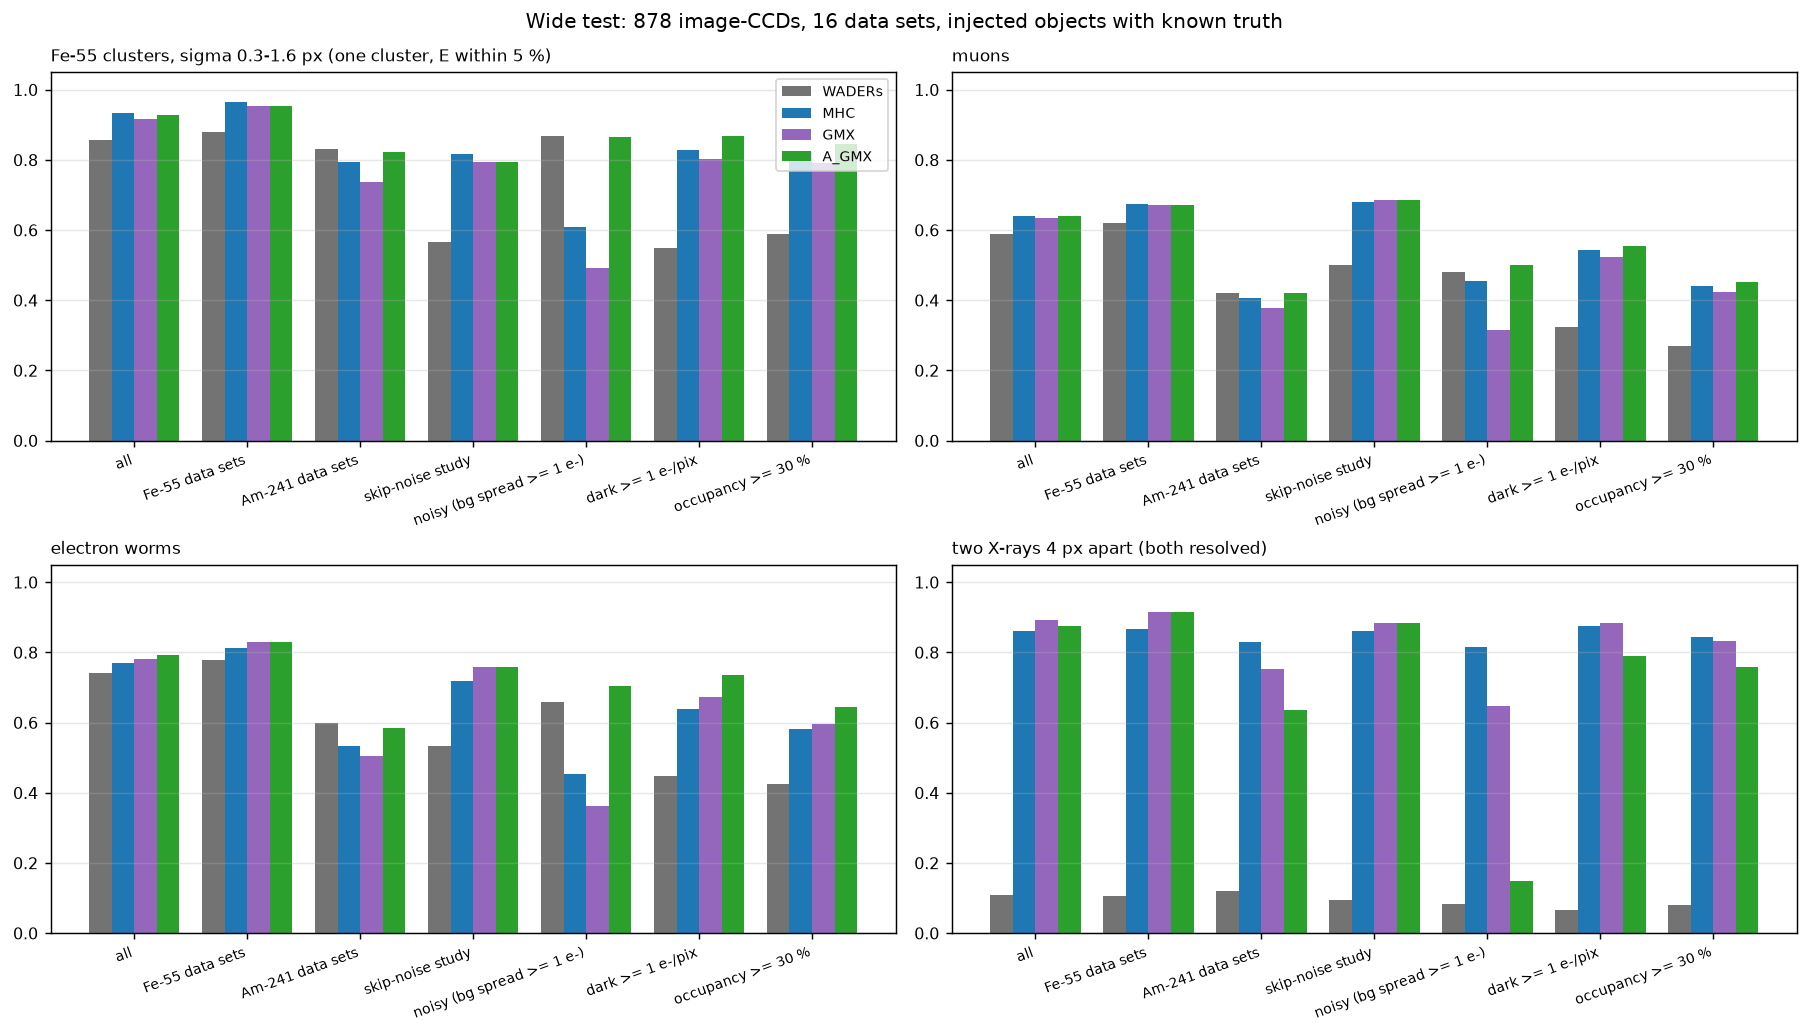
\includegraphics[width=0.92\textwidth]{figures/fig20_wide_vs_waders.png}
\caption{Wide test (878 image-CCDs): success per object type and image condition. Code of 25 October.}
\end{figure}

\begin{figure}[H]\centering
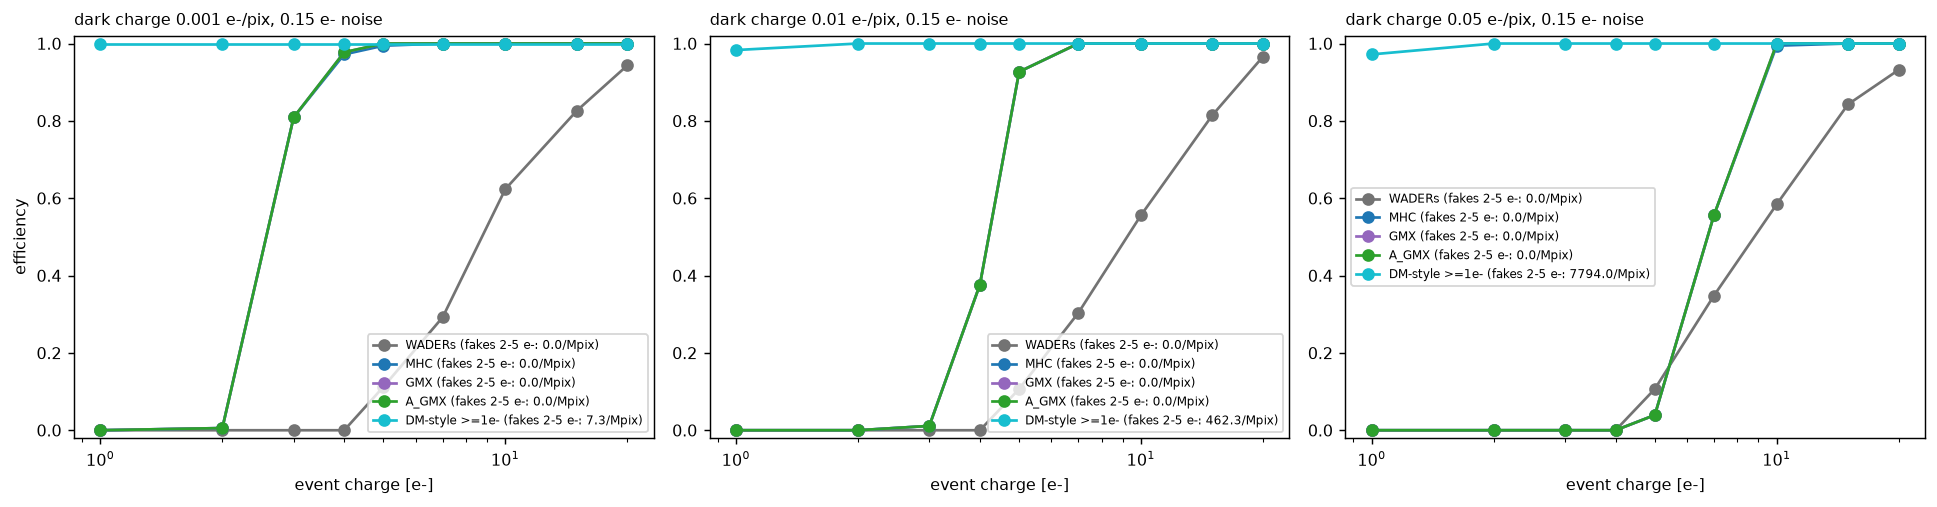
\includegraphics[width=0.92\textwidth]{figures/fig24_few_electron.png}
\caption{Few-electron efficiency against event charge at three dark charges (code of 25 October). WADERs needs
$\gtrsim10$\,\el. The current code's detection background and calibrated threshold raise \AGMX's 3-\el{} efficiency
at the lowest dark charges (table above).}\label{fig:lowe}
\end{figure}

\paragraph{Where WADERs is still the better choice:}
\begin{itemize}
\item speed (about $70\times$ faster);
\item the noisy ``unmodelled'' images (read noise $\ge1$\,\el), where \AGMX{} is WADERs-like hysteresis anyway;
\item hot-column artifacts (0.76 vs 0.74);
\item the smoothness of the crowded-CCD spectrum between the lines (deviance/ndf).
\end{itemize}

\paragraph{Open items:}
\begin{itemize}
\item the higher deviance/ndf on the crowded CCD;
\item thresholds for noisy images (pixel $\ge4.5$\,\el{} is a stop-gap);
\item the background fixes raise the fitted dark charge on the crowded CCD (0.093 $\to$ 0.157\,\el/pix median),
which shifts the 59.5-keV peak by about +0.1\,keV;
\item recalibrating the $\chi^2$ flag for the exact model;
\item rerunning the wide, Fe-55 and track tests on the current code.
\end{itemize}

\end{document}
